
\chapter{Controles}
É possível aumentar e baixar a velocidade usando o botão "up" e "down" do teclado. O avião também pode realizar curvas. 
Isso pode ser feito usando as setas do teclado; quando a seta é solta, o avião volta para o voo nivelado mantendo a proa constante. Enquanto a tecla da direita é pressionada o avião aumenta o ângulo de proa em uma razão constante, enquanto a tecla esquerda é pressionada a proa diminui também em razão constante.

A proa pode variar de 0 graus a 359. Ocorre underflow quando o valor fica menor que zero e overflow quando fica maior que 359.

\begin{verbatim}
    
357        358         359   <-- -1 -- +1 -->  0        1        2
                        
\end{verbatim}

Também é possível usar o mouse; nesse caso, com o cursor na posição central da janela, o voo é mantido nivelado. A distância para a direita ou esquerda determina o quanto a aeronave inclinará para o lado escolhido, permitindo fazer uma curva mais fechada ou aberta. O avião só voltará para o voo nivelado caso o cursor seja recolocado na posição central.

Apenas a coordenada X do mouse importa; a coordenada Y é descartada.

Sendo:

\begin{itemize}
\item W: largura da tela;
\item R\_max: Razão máxima de mudança do ângulo da proa;
\item R: Razão atual de mudança do ângulo da proa;
\item delta: explicado anteriormente;
\item heading: proa atual.
\end{itemize}


A proa atual é calculada por
\texttt{heading += R * delta}

Para se achar o \texttt{R} usa-se a posição x do cursor dentro da tela.

\begin{figure}[h]
    \centering
    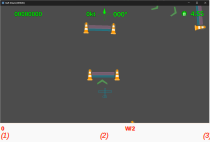
\includegraphics[width=\textwidth]{mouse-x.png}
\end{figure}

\begin{itemize}
\item \textbf{(1)} = cursor no canto esquerdo da janela: \texttt{R = -R\_max}
\item \textbf{(2)} = cursor no meio da janela: \texttt{R = 0}
\item \textbf{(3)} = cursor no canto direito da janela: \texttt{R = R\_max}
\end{itemize}

Para valores entre '1 e 2' e '2 e 3' é feita interpolação linear.
